\documentclass[aspectratio=169, 11pt]{beamer}

\usetheme{Madrid}
\usecolortheme{whale}

\usepackage[utf8]{inputenc}
\usepackage[T1]{fontenc}
\usepackage{booktabs}
\usepackage{tikz}
\usetikzlibrary{arrows.meta, positioning}
\usepackage{amsmath}
\usepackage{amssymb}

\definecolor{accentblue}{RGB}{30,80,160}
\definecolor{accentgreen}{RGB}{20,130,80}
\definecolor{accentorange}{RGB}{200,90,20}
\definecolor{accentred}{RGB}{180,30,30}

% Pipeline-diagram palette, matching the main manuscript's Figure (fig:pipeline)
\definecolor{inputcol}{RGB}{220,220,220}
\definecolor{stagecol}{RGB}{195,225,255}
\definecolor{llmcol}{RGB}{255,210,130}
\definecolor{repaircol}{RGB}{255,252,180}
\definecolor{guardcol}{RGB}{195,240,195}
\definecolor{loopcol}{RGB}{255,200,195}
\definecolor{outputcol}{RGB}{180,210,255}
\definecolor{evalcol}{RGB}{225,200,255}

\setbeamercolor{structure}{fg=accentblue}
\setbeamertemplate{navigation symbols}{}

\title[Robustness Suite Update]{Robustness \& Evaluation Suite}
\subtitle{Progress Update --- Synthagent}
\author{Sancho Amaral Simões}
\date{\today}

\begin{document}

\begin{frame}
\titlepage
\end{frame}

% ------------------------------------------------------------
\begin{frame}{Where We Left Off}
\begin{itemize}
\item Synthagent: agentic LLM pipeline with deterministic guardrails --- 0\% logical violations, exact volume guarantees.
\item Evaluation so far: fidelity dashboard (JSD, correlation, novelty, DCR), 10-fold ML utility benchmark, single-tier ablation design (4 factors, results pending).
\item \alert{Open questions}: Is the benefit specific to one LLM? Was the ``Strategy Ponder'' module itself ever tested? How does it compare to classical baselines under an \emph{identical} protocol?
\end{itemize}
\end{frame}

% ------------------------------------------------------------
\begin{frame}{Architecture Recap: The Synthagent Pipeline}
\begin{center}
\resizebox{\linewidth}{!}{%
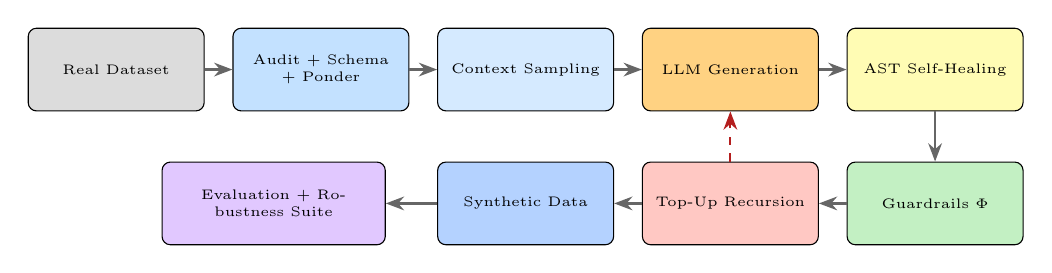
\begin{tikzpicture}[
  every node/.style={font=\tiny, align=center},
  box/.style={rectangle, rounded corners=3pt, draw, minimum height=1.05cm, text width=2.0cm},
  arr/.style={-{Stealth}, thick, draw=black!60},
  farr/.style={-{Stealth}, thick, dashed, draw=accentred}
]
% Row 1: left to right
\node[box, fill=inputcol]                  (data)  at (0,0)    {Real Dataset};
\node[box, fill=stagecol]                  (audit) at (2.6,0)  {Audit + Schema + Ponder};
\node[box, fill=stagecol!70]               (ctx)   at (5.2,0)  {Context Sampling};
\node[box, fill=llmcol]                    (llm)   at (7.8,0)  {LLM Generation};
\node[box, fill=repaircol]                 (ast)   at (10.4,0) {AST Self-Healing};

% Row 2: right to left (wraps back under Row 1)
\node[box, fill=guardcol]                  (phi)   at (10.4,-1.7) {Guardrails $\Phi$};
\node[box, fill=loopcol]                   (topup) at (7.8,-1.7)  {Top-Up Recursion};
\node[box, fill=outputcol]                 (syn)   at (5.2,-1.7)  {Synthetic Data};
\node[box, fill=evalcol, text width=2.6cm] (eval)  at (2.0,-1.7)  {Evaluation \alert{+ Robustness Suite}};

\draw[arr] (data)  -- (audit);
\draw[arr] (audit) -- (ctx);
\draw[arr] (ctx)   -- (llm);
\draw[arr] (llm)   -- (ast);
\draw[arr] (ast)   -- (phi);
\draw[arr] (phi)   -- (topup);
\draw[arr] (topup) -- (syn);
\draw[arr] (syn)   -- (eval);
\draw[farr] (topup.north) -- (llm.south);
\end{tikzpicture}%
}
\end{center}
\vspace{0.2cm}
\footnotesize
\begin{itemize}
\item Deterministic guardrails + Top-Up Recursion (dashed feedback) $\Rightarrow$ exact volume, 0\% logical violations.
\item \alert{Evaluation} now includes the new Robustness Suite --- everything on the following slides.
\end{itemize}
\end{frame}

% ------------------------------------------------------------
\begin{frame}{What's New: Two-Tier Robustness Suite}
\begin{center}
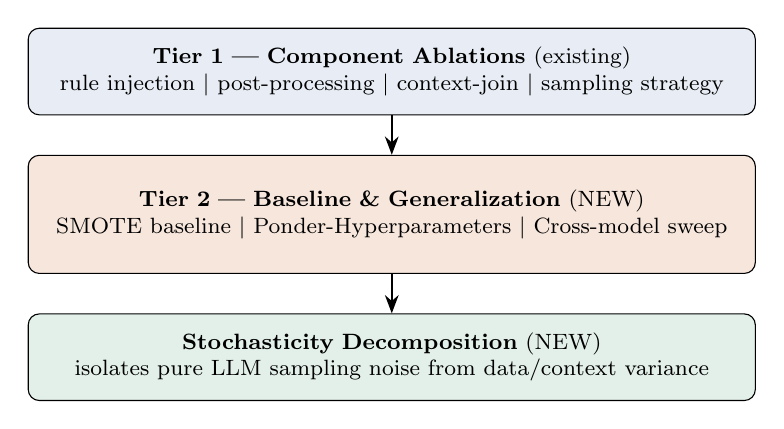
\begin{tikzpicture}[node distance=0.5cm, every node/.style={font=\footnotesize}]
\node[draw, fill=accentblue!10, rounded corners, text width=9cm, align=center, minimum height=1.1cm]
  (t1) {\textbf{Tier 1 --- Component Ablations} (existing)\\ rule injection \textbar\ post-processing \textbar\ context-join \textbar\ sampling strategy};
\node[draw, fill=accentorange!15, rounded corners, text width=9cm, align=center, minimum height=1.5cm, below=of t1]
  (t2) {\textbf{Tier 2 --- Baseline \& Generalization} \alert{(NEW)}\\ SMOTE baseline \textbar\ Ponder-Hyperparameters \textbar\ Cross-model sweep};
\node[draw, fill=accentgreen!12, rounded corners, text width=9cm, align=center, minimum height=1.1cm, below=of t2]
  (st) {\textbf{Stochasticity Decomposition} \alert{(NEW)}\\ isolates pure LLM sampling noise from data/context variance};
\draw[-{Stealth}, thick] (t1) -- (t2);
\draw[-{Stealth}, thick] (t2) -- (st);
\end{tikzpicture}
\end{center}
\end{frame}

% ------------------------------------------------------------
\begin{frame}{NEW Arm 1: SMOTE Baseline, Same Harness}
\begin{itemize}
\item Previously: SMOTE comparison used \alert{literature-published numbers} on different splits.
\item Now: SMOTE/SMOTENC runs \alert{through our own 10-fold harness} --- identical seeds, identical ML evaluation.
\item Categorical features handled via SMOTENC; $k_{\text{neighbors}} = \min(5,\, n_{\min}-1)$.
\item Found \& fixed a real bug: SMOTE's synthetic output is single-class by construction $\Rightarrow$ the ``generated-only'' ML arm is degenerate for SMOTE --- but original-vs-augmented must not be discarded because of it.
\item Near-zero generation cost vs.\ LLM --- now quantified explicitly, per fold.
\end{itemize}
\end{frame}

% ------------------------------------------------------------
\begin{frame}{NEW Arm 2: Structured Ponder-Hyperparameters}
\begin{itemize}
\item Strategy Ponder is named as a core contribution in the abstract --- but was \alert{never empirically tested}.
\item Added a structured counterpart: the LLM returns strict JSON $\hat\Theta = (\hat\alpha, \hat s, \hat\tau)$ instead of free text.
\item Each field validated independently; invalid or missing fields fall back to safe defaults --- never crashes the run.
\item New ablation arm: run the pipeline with $\hat\Theta$ instead of fixed defaults, compare against \texttt{full}.
\end{itemize}
\end{frame}

% ------------------------------------------------------------
\begin{frame}{NEW Arm 3: Cross-Model Sweep (Live-Discovered)}
\begin{itemize}
\item Question: does the framework's benefit generalize beyond one LLM?
\item \alert{No hardcoded model list.} At run time, queries the inference server's \texttt{/v1/models} endpoint.
\item Automatically excludes the default model (covered by other arms) and embedding-only models.
\item One arm per discovered chat-capable model --- the arm set grows or shrinks automatically as models are loaded/unloaded, no code change needed.
\item Verified live: correctly found \texttt{qwen2.5-vl-7b-instruct}, correctly skipped the embedding model.
\end{itemize}
\end{frame}

% ------------------------------------------------------------
\begin{frame}{NEW Privacy Metrics: C2ST + MIA}
\begin{itemize}
\item Previously: privacy metrics (DCR, Privacy Risk) computed on our own data, but C2ST/MIA only \alert{cited for competitors}.
\item Now computed on \emph{our own} synthetic data:
\begin{itemize}
\item \textbf{C2ST}: a classifier trained to distinguish real vs.\ synthetic rows. $\approx 0.5$ = indistinguishable.
\item \textbf{MIA}: a nearest-neighbour distance attack, scored via ROC-AUC. $\approx 0.5$ = no membership leakage.
\end{itemize}
\item Both degrade gracefully to ``not reported'' on too-small folds, rather than a misleading number.
\end{itemize}
\end{frame}

% ------------------------------------------------------------
\begin{frame}{Other New Evaluation Machinery}
\begin{itemize}
\item \textbf{Per-class fidelity}: every fidelity metric recomputed separately on minority/majority class --- does synthetic quality hold up where it matters most?
\item \textbf{Multiple-comparison correction}: Benjamini--Hochberg FDR control across every (arm, metric) test family --- avoids false positives from running hundreds of tests.
\item \textbf{Stochasticity decomposition}: fixes ONE split + ONE context sample, repeats generation $R{=}5$ times $\Rightarrow$ isolates pure LLM sampling noise.
\item \textbf{Per-fold wall-clock timing}: tracked for every fold, every arm --- powers the SMOTE-vs-LLM cost contrast.
\end{itemize}
\end{frame}

% ------------------------------------------------------------
\begin{frame}{Engineering: Checkpoint \& Resume}
\begin{itemize}
\item The robustness suite now spans $\sim$540 runs --- long enough that a crash, kill, or LLM timeout mid-run is a real risk (we hit exactly this during testing).
\item Every completed unit is checkpointed to disk immediately (atomic write).
\item Re-running with \texttt{--resume} skips completed units, recomputes only what's missing.
\item Safety check: a resumed run only reuses a cached unit if it was produced with the \alert{same fold count} --- otherwise it's recomputed, never silently mixed.
\end{itemize}
\end{frame}

% ------------------------------------------------------------
\begin{frame}{Scale: Before vs.\ After}
\centering
\footnotesize
\begin{tabular}{lcc}
\toprule
 & \textbf{Before} & \textbf{After} \\
\midrule
Ablation arms          & 6 (Tier 1 only)      & 9 (Tier 1 + Tier 2) \\
Privacy metrics        & DCR, Privacy Risk    & + C2ST, MIA \\
Fidelity granularity   & pooled only          & + per-class (min/maj) \\
Significance testing   & raw $p$-values       & + BH-corrected $q$-values \\
Stochasticity isolation & none                & dedicated decomposition \\
Total runs             & $\sim$60 (main)      & $\sim$540 (full suite) \\
Fault tolerance        & none                 & checkpoint / resume \\
\bottomrule
\end{tabular}
\end{frame}

% ------------------------------------------------------------
\begin{frame}{Status \& Next Steps}
\begin{itemize}
\item \textcolor{accentgreen}{\textbf{Done:}} All mechanisms implemented, unit-tested (164 tests passing), verified live against LM Studio.
\item \textcolor{accentgreen}{\textbf{Done:}} Manuscript formalizes every new arm, metric, and protocol --- results deferred, not fabricated.
\item \textcolor{accentorange}{\textbf{Next:}} Execute the full $\sim$540-run sweep and report FDR-corrected results in the next revision.
\item \textcolor{accentorange}{\textbf{Discuss:}} Prioritize the full Tier 1+2 sweep, or a faster representative subset first?
\end{itemize}
\end{frame}

% ------------------------------------------------------------
\begin{frame}
\centering
\Large Questions / Discussion
\end{frame}

\end{document}
